\documentclass[12pt, a4paper]{article}

\usepackage[english]{babel} 
\usepackage[T1]{fontenc}
\usepackage{amsfonts} 
\usepackage{setspace}
\usepackage{amsmath}
\usepackage{amssymb}
\usepackage{tikz}

\graphicspath{./}

\newcommand*{\qed}{\null\nobreak\hfill\ensuremath{\square}}
\newcommand*{\puffer}{\text{ }\text{ }\text{ }\text{ }}
\newcommand*{\lhop}{\mathrel{\overset{\makebox[0pt]{\mbox{\normalfont\tiny\sffamily l'hop.}}}{=}}}

\pagestyle{plain}
\allowdisplaybreaks

\title{Computer Networks - Assignment 9}
\author{Jannis Kühl, Henri Heyden\\ \small stu241399, stu240825}
\date{}


\begin{document}
\maketitle
\section*{Task 1}
\subsection*{a)}
We marked the predecessors for the shortest paths in the following image:
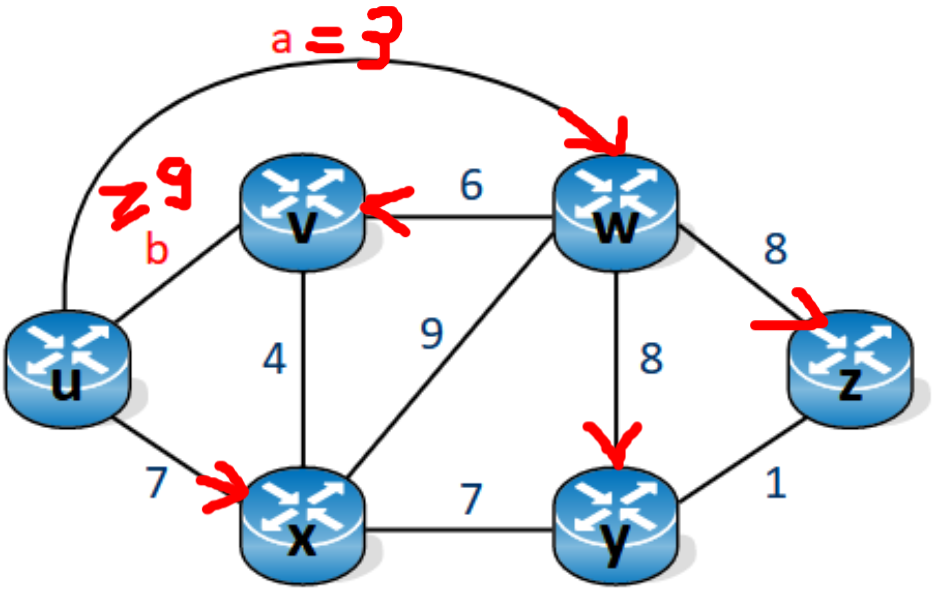
\includegraphics[width=\textwidth]{A1.png}
Because the table states that the shortest path from u to w is a direct connection, we can set a to 3, because a is the wheight of the connection between u to w. \\
Since we also know that the shortest path to v has its predecessor as w, and we know the shortest path to w, which is u->w with wheight 9, we know b must be bigger or equal to 9. \pagebreak
\subsection*{b)}
\textbf{1:} Distance vectors before x is added \\ \\
    \begin{tabular}{||c c c c||} 
     \hline
     Destination & dv(u) & dv(v) & dv(w) \\ [0.5ex] 
     \hline\hline
     u & 0 & 2 & 6 \\ 
     \hline
     v & 2 & 0 & 4 \\
     \hline
     w & 6 & 4 & 0 \\
     \hline
    \end{tabular} \\ \\ \\
\textbf{2:} Initial distance vector of x \\ \\
    \begin{tabular}{||c c||} 
     \hline
     Destination & dv(x) \\ [0.5ex] 
     \hline\hline
     u & \(+\infty\) \\ 
     \hline
     v & 2 \\
     \hline
     w & 1 \\
     \hline
     x & 0 \\
     \hline
    \end{tabular} \\ \\ \\
\textbf{3:} Distance vector of x after receiving distance vectors of v and w \\ \\
    \begin{tabular}{||c c||} 
     \hline
     Destination & dv(x) \\ [0.5ex] 
     \hline\hline
     u & 4 \\ 
     \hline
     v & 2 \\
     \hline
     w & 1 \\
     \hline
     x & 0 \\
     \hline
    \end{tabular} \\ \\ \\
\textbf{4:} Distance vectors of v, w after receiving the new distance vector of x \\ \\
    \begin{tabular}{||c c c||} 
     \hline
     Destination & dv(v) & dv(w) \\ [0.5ex] 
     \hline\hline
     u & 2 & 5 \\ 
     \hline
     v & 0 & 3 \\
     \hline
     w & 3 & 0 \\
     \hline
     x & 2 & 1 \\
     \hline
    \end{tabular} \\ \\ \\

\end{document}